\documentclass[10pt]{article}


\usepackage[utf8]{inputenc}
\usepackage[T1]{fontenc}
\usepackage[frenchb]{babel}

\usepackage{algorithm}
\usepackage{algorithmic}
\usepackage[T1]{fontenc}
\usepackage{enumitem}
\usepackage{hyperref}
\usepackage{graphicx}
\usepackage{color}
\usepackage{listings}
\usepackage{wrapfig}
\usepackage{amsfonts}
\usepackage{amsmath}
\usepackage{mathtools}
\usepackage[hmargin=1.25in,vmargin=1.25in]{geometry}
\usepackage{framed}
\usepackage{mathenv}
\usepackage{blkarray}

%title setuplisting
\title{MPM2 Projet Mathématique 2017-2018}
\author{
  Etienne TAILLEFER DE LAPORTALIERE \\
  Romain PEREIRA\\
  Cyril PIQUET
}
\date{13/02/2018}

% table of contents setup
\renewcommand{\contentsname}{Sommaire}
\usepackage{etoolbox}
\patchcmd{\thebibliography}{\section*{\refname}}{}{}{}

% systeme d'équation
\newenvironment{sistema}%
{\left\lbrace\begin{array}{@{}l@{}}}%
  {\end{array}\right.}

\setlength{\parindent}{0cm}
\setlength{\parskip}{1ex plus 0.5ex minus 0.2ex}
\newcommand{\hsp}{\hspace{20pt}}
\newcommand{\HRule}{\rule{\linewidth}{0.5mm}}

\hypersetup{
  colorlinks,
  citecolor=black,
  filecolor=black,
  linkcolor=blue,
  urlcolor=red
}

\lstset
{ %Formatting for code in appendix
  language=Python,
  basicstyle=\footnotesize,
  numbers=left,
  stepnumber=1,
  showstringspaces=false,
  tabsize=1,
  breaklines=true,
  breakatwhitespace=false,
}
\begin{document}
  
  \begin{titlepage}
    \begin{sffamily}
      \begin{center}
	
	\textsc{\LARGE ENSIIE}\\[2cm]
	\textsc{\Large Rapport de projet Mathématique}\\[1.5cm]
	% Title
	\HRule \\[0.4cm]
	{ \huge \bfseries Projet de Mathématique en groupe (MPM2)\\[0.4cm] }
	\HRule \\[2cm]
	
	\begin{minipage}{0.4\textwidth}
	  \begin{flushleft} \large
	    Romain \textsc{Pereira}\\
	    Cyril \textsc{Piquet}\\
	    Etienne \textsc{Taillefer de Laportalière}\\
	  \end{flushleft}
	\end{minipage}
	\begin{minipage}{0.4\textwidth}
	  \begin{flushright} \large
	    \emph{Enseignants :} \\
	    M. \textsc{Rasamoely}\\
	    M. \textsc{Pulido}\\
	    M. \textsc{Torri}\\
	    M. \textsc{Lim}\\
	  \end{flushright}
	\end{minipage}
	
	\vfill
	% Bottom of the page
	{\large 03/04/2018}
      \end{center}
    \end{sffamily}
  \end{titlepage}
  \maketitle
  \tableofcontents
  
  \section*{Préambule}
  Ce projet est réalisé dans le cadre de nos études à l'ENSIIE.
  L'objectif est de modéliser un marché financier et de déterminer les prix et la couverture d'option européenne.
  \newpage
  \section{Modèle de Cox-Ross-Rubinstein}
  On a \( \boxed{l = 2^N} \) trajectoire possible pour l'évolution du prix de l'actif risqué, entre l'instant initial 1 et l'instant final N.
  \newline
  On a \( \boxed{N + 1}   \) valeurs possibles pour \( S^{N}_{t_N} \)\newline
  \newline
  \paragraph{1.} \(\mathbb{Q}\) est la probabilité risque-neutre, vérifiant: \( \mathbb{E}_{\mathbb{Q}}[T^{(N)}_{1}] = 1 + r_N \)
  \newline
  On note: \( q_n = \mathbb{Q}(T^{(N)}_1 = 1 + h_N) \)
  Donc:
  \begin{equation}
    \begin{split}
      \mathbb{E}_{\mathbb{Q}}[T^{(N)}_1] &= \sum_{t \in T^{(N)}_{1}(\Omega)}x 	\mathbb{P}(T^{(N)}_{1} = t) \\
      \qquad &= (1 + h_n) q_N + (1 + b_n) (1 - q_n) \\
      \qquad &= 1 + r_N \\					
      \qquad \Rightarrow \quad \Aboxed{q_N &= \frac{r_N - b_N}{h_N - b_N}}
    \end{split}
  \end{equation}
  
  \paragraph{2.} Soit \(   p_(N) = \frac{1}{(1 + r_N)^N} \mathbb{E}_{\mathbb{Q}}[f(S^{(N)}_{t_N})]   \),
  le prix de l'option qui paye \( f(S^{(N)}_{t_N}) \).
  \newline
  On a:
  \begin{equation}
    \begin{split}
      \bullet \qquad p_{(0)} 	&= f(s) \\
      \bullet \qquad p_{(1)} 	&= \frac{1}{(1 + r_N)^1} \mathbb{E}_{\mathbb{Q}}[f(S^{(N)}_{t_1})] \\
      &= \frac{1}{(1 + r_N)^1} \mathbb{E}_{\mathbb{Q}}[f(T^{(N)}_{1} S^{(N)}_{t_0})] \\
      &= \frac{1}{1 + r_N} [ q_N f[(1 + h_N)  s] + (1 - q_N) f[(1 + b_N)  s)] ] \\
      &= [...] \text{ (en se basant sur l'arbre de la figure 1)}\\
      \bullet \qquad  \Aboxed{ p_{(N)} 	&= \frac{1}{(1 + r_N)^N} \sum^{N}_{k = 0} {N\choose k} q_N^k (1 - q_N)^{N - k} f((1 + h_N)^k (1 + b_N)^{N - k} s)}
    \end{split}
  \end{equation}
  
  \newpage
  \subsection{Premier pricer}
  \paragraph{Code python du 1er pricer.} Le code est disponible dans le fichier 'code/pricer.py' et 'code/Premier\_pricer.py'
  
  \paragraph{3.} voir ligne 8 à 27 du fichier `code/Q3.py`
  
  \paragraph{4.} voir ligne 6 du fichier `code/Q4.py`
  
  La fonction renvoie '18.5686591182' pour ces paramètres.

  \begin{figure}[H]
    \begin{center}
      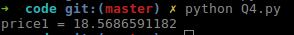
\includegraphics[height=1cm,keepaspectratio]{./images/q4.png}
    \end{center}
    \caption{\textit{Résultat price1}}
    \label{q4}
  \end{figure}
  
  
  \subsection{Deuxième pricer}    
  Nous allons utiliser un algorithme de calcul récursif. 
  
  Ici on a:
  \begin{alignat*}{2}
    \forall k \in \mathbb{N}, \quad \mathbb{E}_{\mathbb{Q}}[v_{k+1}(S^{(N)}_{k + 1}) \slash S^{(N)}_k] 	&= \sum_{S \in(S^{(N)}_{k + 1} \slash S^{(N)}_k)(\Omega)} v_{k+1}(S) \mathbb{P}((S^{(N)}_{k + 1} \slash S^{(N)}_{k}) = S)\\
													& = \boxed{v_{k+1}((1 + r_n)S^{(N)}_{k})q_n + v_{k+1}((1 + b_n)S^{(N)}_{k})(1 - q_n)} \\
    v_k(S_{t_k}^{N}) \quad \quad \quad \quad \quad \quad &= \frac{{E}_{\mathbb{Q}}[v_{k+1}(S^{(N)}_{k + 1}) \slash S^{(N)}_k]}{1+r_N} \\
    v_N(S_{t_N}^{N}) \quad \quad \quad \quad \quad \quad &= f(S_{t_k}^{N})
  \end{alignat*}
  Donc, $$\boxed{v_k(S_{t_k}^{N})=\frac{{v_{k+1}((1 + r_n)S^{(N)}_{k})q_n + v_{k+1}((1 + b_n)S^{(N)}_{k})(1 - q_n)} }{1+r_N}}$$

  On peut alors remonter avec une récursion montante (connaissant l'etat final).
  
  \paragraph{Code python du 2eme pricer.}
  
  \paragraph{5.} voir ligne 32 à 39 du fichier `code/Q5.py`
  
  \paragraph{6.} voir ligne 6 du fichier `code/Q6.py`
  
  La fonction renvoie '10.7573397487' pour ces paramètres.
  
  \begin{figure}[H]
    \begin{center}
      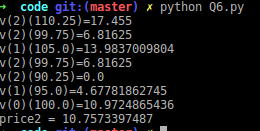
\includegraphics[height=5cm,keepaspectratio]{./images/q6.png}
    \end{center}
    \caption{\textit{Résultat price2}}
    \label{q6}
  \end{figure}
  
  \begin{figure}[H]
    \begin{center}
      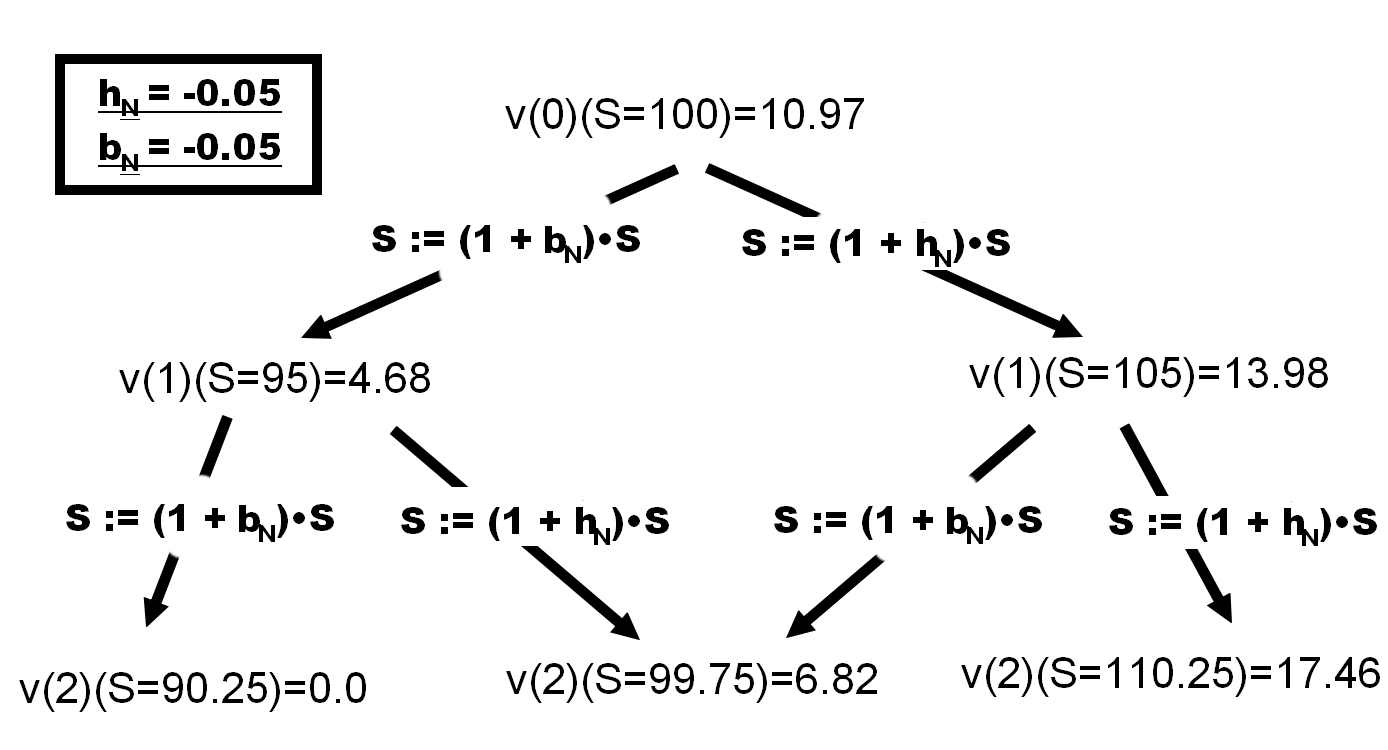
\includegraphics[height=6cm,keepaspectratio]{./images/q6_tree.png}
    \end{center}
    \caption{\textit{Résultat price1}}
    \label{q6_tree}
  \end{figure}
  
  \subsection{Comparaison}
  \paragraph{7.}
  Pour ces entrées, (et pour toutes valeurs de N dans $\mathbb{[}5, 15\mathbb{]}$ les fonctions \textit{price1} et \textit{price2}
  renvoient les mêmes prix (à $10^{-11}$ prêt).
  
  Voici un résultat obtenu, pour $N=11$
    \begin{figure}[H]
      \begin{center}
	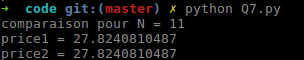
\includegraphics[height=2cm,keepaspectratio]{./images/q7.png}
      \end{center}
      \caption{\textit{Comparaison price1 et price2}}
      \label{q7}
    \end{figure}
    
  \subsection{La couverture}
  \paragraph{8.}
  $$
  \begin{sistema}
    \alpha_{N-1}(S^{(N)}_{t_{N-1}})*(1+h_N)*S^{(N)}_{t_{N-1}} + \beta_{N-1} (S^{(N)}_{t_{N-1}})*S^{(0)}_{t_{N}}=f( (1+h_N)*S^{(N)}_{t_{N-1}}) \quad \quad (L_1)\\
    \alpha_{N-1}(S^{(N)}_{t_{N-1}})*(1+b_N)*S^{(N)}_{t_{N-1}} + \beta_{N-1} (S^{(N)}_{t_{N-1}})*S^{(0)}_{t_{N}}=f( (1+b_N)*S^{(N)}_{t_{N-1}}) \quad \quad (L_2)
  \end{sistema}
  $$
  
  $$
  (L_2) - (L_1) : \alpha_{N-1}(S^{(N)}_{t_{N-1}}) * S^{(N)}_{t_{N-1}} * (h_N - b_N) = f( (1+h_N)*S^{(N)}_{t_{N-1}}) - f( (1+b_N)*S^{(N)}_{t_{N-1}})
  $$
  
  Donc :
  $$
  \boxed{\alpha_{N-1}(S^{(N)}_{t_{N-1}}) = \frac{f( (1+h_N)*S^{(N)}_{t_{N-1}}) - f( (1+b_N)*S^{(N)}_{t_{N-1}})}{S^{(N)}_{t_{N-1}} * (h_N - b_N)}}
  $$
  \newline
  \newline
  On injecte le résultat précédent dans $(L_1)$ :
  
  \begin{align}
     \frac{f( (1+h_N)*S^{(N)}_{t_{N-1}}) - f( (1+b_N)*S^{(N)}_{t_{N-1}})}{(h_N - b_N)}*(1+h_N) + \beta_{N-1} (S^{(N)}_{t_{N-1}})*S^{(0)}_{t_{N}}\\
      = f( (1+h_N)*S^{(N)}_{t_{N-1}}) 
  \end{align}
  Donc:
  $$
  \beta_{N-1} (S^{(N)}_{t_{N-1}})*(1+r_N)^N = \frac{(h_N - b_N)*f( (1+h_N)*S^{(N)}_{t_{N-1}}) - f( (1+h_N)*S^{(N)}_{t_{N-1}}) + f( (1+b_N)*S^{(N)}_{t_{N-1}})}{(h_N - b_N)}
  $$
  D'où :
  $$
  \boxed{\beta_{N-1} (S^{(N)}_{t_{N-1}}) = \frac{(1+h_N)*f( (1+b_N)*S^{(N)}_{t_{N-1}}) - (1+b_n)*f( (1+h_N)*S^{(N)}_{t_{N-1}})}{(h_N - b_N)*(1+r_N)^N}}
  $$
  
  \paragraph{9.}
  $$
  \begin{sistema}
    \alpha_{k-1}(S^{(N)}_{t_{k-1}})*(1+h_N)*S^{(N)}_{t_{k-1}} + \beta_{k-1} (S^{(N)}_{t_{k-1}})*S^{(0)}_{t_{k}}=v_{k}( (1+h_N)*S^{(N)}_{t_{k-1}}) \quad \quad (L_1)\\
    \alpha_{k-1}(S^{(N)}_{t_{k-1}})*(1+b_N)*S^{(N)}_{t_{k-1}} + \beta_{k-1} (S^{(N)}_{t_{k-1}})*S^{(0)}_{t_{k}}=v_{k}( (1+b_N)*S^{(N)}_{t_{k-1}}) \quad \quad (L_2)
  \end{sistema}
  $$
  
  De la même manière on obtient :
  $$
    \boxed{\alpha_{k-1}(S^{(N)}_{t_{k-1}}) = \frac{v_{k}( (1+h_N)*S^{(N)}_{t_{k-1}}) - v_{k}( (1+b_N)*S^{(N)}_{t_{k-1}})}{S^{(N)}_{t_{k-1}} * (h_N - b_N)}}
  $$
  
  $$
    \boxed{\beta_{k-1} (S^{(N)}_{t_{k-1}}) = \frac{(1+h_N)*v_{k}( (1+b_N)*S^{(N)}_{t_{k-1}}) - (1+b_n)*v_{k}( (1+h_N)*S^{(N)}_{t_{k-1}})}{(h_N - b_N)*(1+r_N)^N}}
  $$
  
  \paragraph{10.} voir code dans le fichier 'code/Q10.py'
  
  Pour la date 0 la couverture a pour expression:
  $$
    \boxed{\alpha_{0}(S^{(2)}_{t_{0}}) = \frac{v_{1}( (1+h_N)*S^{(2)}_{t_{0}}) - v_{1}( (1+b_N)*S^{(2)}_{t_{0}})}{S^{(2)}_{t_{0}} * (h_N - b_N)}}
  $$
  
  $$
    \boxed{\beta_{k-1} (S^{(N)}_{t_{k-1}}) = \frac{(1+h_N)*v_{k}( (1+b_N)*S^{(N)}_{t_{k-1}}) - (1+b_n)*v_{k}( (1+h_N)*S^{(N)}_{t_{k-1}})}{(h_N - b_N)*(1+r_N)^N}}
  $$
  
  avec ici $S^{(2)}_{t_{0}}=100$ et $V_{1}(S_{t0}^{(2)})= \frac{\mathbb{E}_{\mathbb{Q}}[f(S_{t1}^{(2)}) \slash S_{t0}^{(2)}]}{1+r_N}=\frac{f((1+h_N)S_{t0}^{(2)})q_N + f((1+b_N)S_{t0}^{(2)})(1-q_N)}{1+r_N}$
  Ainsi avec ces paramètres on trouve pour la couverture à la date t=0:
  $\alpha_0(100)=0.79$ et $\beta_0(100)=-78$
  
  Pour la couverture à la date t1 il y a deux cas:
  Soit $S_{t1}^{(2)}=S_{t0}^{(2)}(1+h_N)=s(1+h_N)=105$ soit $S_{t1}^{(2)}=S_{t0}^{(2)}(1+b_N)=s(1+b_N)=95$
  Il faut donc traiter ces deux cas:
  Dans les deux cas on a la couverture suivante à la date 1:
  $$
  \boxed{\alpha_{1}(S^{(2)}_{t_{1}}) = \frac{f( (1+h_N)*S^{(2)}_{t_{1}}) - f( (1+b_N)*S^{(2)}_{t_{1}})}{S^{(2)}_{t_{1}} * (h_N - b_N)}}
  $$
  $$
  \boxed{\beta_{1} (S^{(2)}_{t_{1}}) = \frac{(1+h_N)*f( (1+b_N)*S^{(2)}_{t_{1}}) - (1+b_N)*f( (1+h_N)*S^{(2)}_{t_{1}})}{(h_N - b_N)*(1+r_N)^2}}
  $$
  Ainsi avec ces paramètres on trouve pour la couverture à la date t=1:
  
  Si   $S_{t1}^{(2)}=105$    $\alpha_1(105)=0.97$ et $\beta_1(105)=-91.35$
  
  Si   $S_{t1}^{(2)}=95$    $\alpha_1(95)=0$ et $\beta_1(95)=0$
  
  \section{Modèle de Black-Scholes}
  \subsection{Le modèle}
  \paragraph{11.}
  On sait que pour toutes fonctions $g \in {C^2} $ on a la formule d'Ito suivante :
  
  $$ dg(S_t) = g'(S_t)dS_t + \frac{|\sigma S_t|^2}{2}g''(S_t)dt $$
  
  On applique la formule d'Ito à à $ln(S_t)$
  
  
  \begin{align*}
    d\ln(S_t) &= \frac{1}{S_t}dS_t + \frac{|\sigma S_t|^2}{2}\frac{-1}{S_t^2}dt \\
    \Rightarrow \frac{d\ln(S_t)}{dt} &= \frac{1}{S_t}\frac{dS_t}{dt} + \frac{|\sigma S_t|^2}{2}\frac{-1}{S_t^2}
  \end{align*}
  
  Or on a $ d(S_t) = S_t(rdt + \sigma d \beta_t)$
  
  Donc :
  
  $$ \frac{d\ln(S_t)}{dt} = r + \frac{1}{S_t}\frac{\sigma d \beta_t}{dt} + \frac{|\sigma S_t|^2}{2}\frac{-1}{S_t^2} $$
  
  On intègre alors la formule précédente (avec la constante en 0 : s) :
  
  $$ \ln(S_t) = \ln(s) + rt + \sigma \beta_t - \frac{\sigma^2}{2}t $$
  
  On a donc :
  
  $$ S_t = s\exp^{rt + \sigma \beta_t - \frac{\sigma^2}{2}t} $$
  $$ \Rightarrow \boxed{S_t = s\exp^{\sigma \beta_t + (r-\frac{\sigma^2}{2})t}} $$
  
  \subsection{Le pricer par la méthode de Monte-Carlo}
  \paragraph{12.}La formule est explicite dans le sujet, on utilise la fonction rnorm pour le $\epsilon_i$.  Voir fichier `code/Q12.py`
  
  \paragraph{13.} voir fichier `code/Q13.py`
  
  \begin{figure}[H]
    \begin{center}
      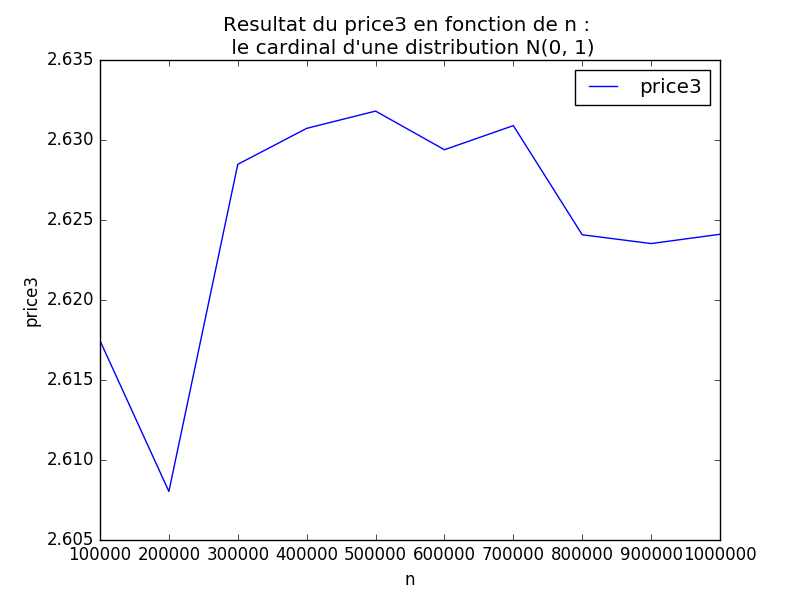
\includegraphics[height=9cm,keepaspectratio]{./images/q13.png}
    \end{center}
    \caption{\textit{Graphique du pricer3 en fonction de 'n'}}
    \label{q13}
  \end{figure}
  
  \paragraph{14.} Montrons que $ (\hat{p}(n)) $ converge presque sûrement vers p:
  
  On a: $$\hat{p}(n) = \frac{1}{n} \sum_{i=1}^n \exp^{-rT}f(s\exp^{(r-\frac{\sigma^2}{2})T + \sigma \sqrt{T}\xi_i})$$
  
  Pour répondre à cette question, nous allons utiliser la loi des grands nombres.
  
  \paragraph{Loi des grands nombres} Soit $(X_i)$ une suite de variables intégrables indépendantes 2 à 2 identiquement distribuées, on a alors :
  $ \bar{X_n}$ converge presque surement vers $ \bar{\mu_n} $ avec $ \bar{X_n} = \frac{1}{n} \sum_1^n X_i $ et $ \bar{\mu_n} = E[X_1] $
  
  On note $X_i = \exp^{-rT}f(s\exp^{(r-\frac{\sigma^2}{2})T + \sigma \sqrt{T}\xi_i})$
  Or d'après le sujet les $(\delta_i)$ sont une suite de variables indépendantes et identiquement distribuées
  Donc les $X_i$ respectent les conditions de la loi des grands nombres.
  
  Donc $\hat{p}(n)$ converge presque surement vers $E[X_1]$
  
  Or $E[X_1] = E[exp^{-rT}f(s\exp^{(r-\frac{\sigma^2}{2})T + \sigma \sqrt{T}\xi_i})]$
  
  De plus on sait que : $p = E[\exp^{-rt}f(S_t)]$
  
  Or d'après la question 12 on a :
  $ p = E[exp^{-rT}f(s\exp^{(r-\frac{\sigma^2}{2})T + \sigma \beta_T}] $
  avec $\beta_T$ un mouvement Brownien donc $ \forall s \in [0,T] $ on a donc $\beta_t - \beta_s \sim N(0,t-s) $. Donc pour s=0 on a : $ \beta_T \sim N(0,T) $
  
  Et donc $ \frac{\beta_T}{\sqrt{T}} \sim N(0,1) $ donc on peut noter $ \xi_1 = \beta_t \sqrt{t} \sim N(0,1) $
  
  En faisant ce remplacement p devient:
  $$p = E[exp^{-rT}f(s\exp^{(r-\frac{\sigma^2}{2})T + \sigma \sqrt{T}\xi_i})]$$
  $$p=E[X_1]$$
  Donc $$\boxed {\hat{p}(n) \text{converge presque surement vers } p}$$
  
  \newpage
  \subsection{Le pricer par formule fermée}
  \paragraph{15.} La formule est explicite dans le sujet, on utilise la fonction norm.cdf pour la fonction de répartition.
  Voir fichier `code/Q15.py`
  
  \paragraph{16.} voir fichier `code/Q16.py`
    \begin{figure}[H]
      \begin{center}
	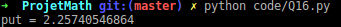
\includegraphics[height=0.8cm,keepaspectratio]{./images/q16.png}
      \end{center}
      \caption{\textit{Price3 en fonction de 'n', et 'put'}}
      \label{q16}
    \end{figure}
    
  \paragraph{17.} voir fichier `code/Q17.py`
  On remarque que la fonction \textit{price3} oscille autour du prix \textit{put}, et semble converger vers le prix \textit{put}.
  
  
  Ce graphe confirme ainsi la théorie de la question 14, la suite $p_n$ converge presque surement vers p.
  \begin{figure}[H]
    \begin{center}
      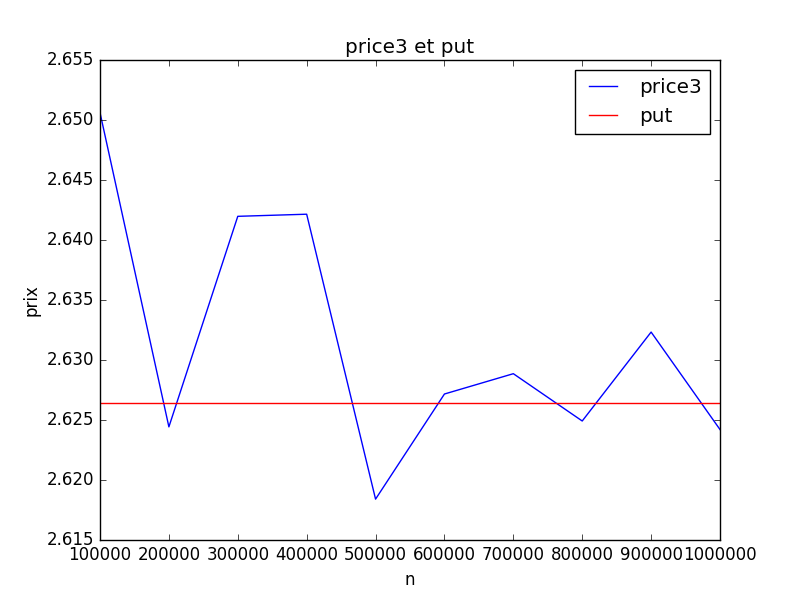
\includegraphics[height=9cm,keepaspectratio]{./images/Q17.png}
    \end{center}
    \caption{\textit{Price3 en fonction de 'n', et 'put'}}
    \label{Q17}
  \end{figure}
  
  \paragraph{18.} voir fichier `code/Q18.py`
  On remarque que le prix du put ne dépend pas du temps mais que de s. Ainsi le prix du put est indépendant du temps.
  
  \begin{figure}[H]
    \begin{center}
      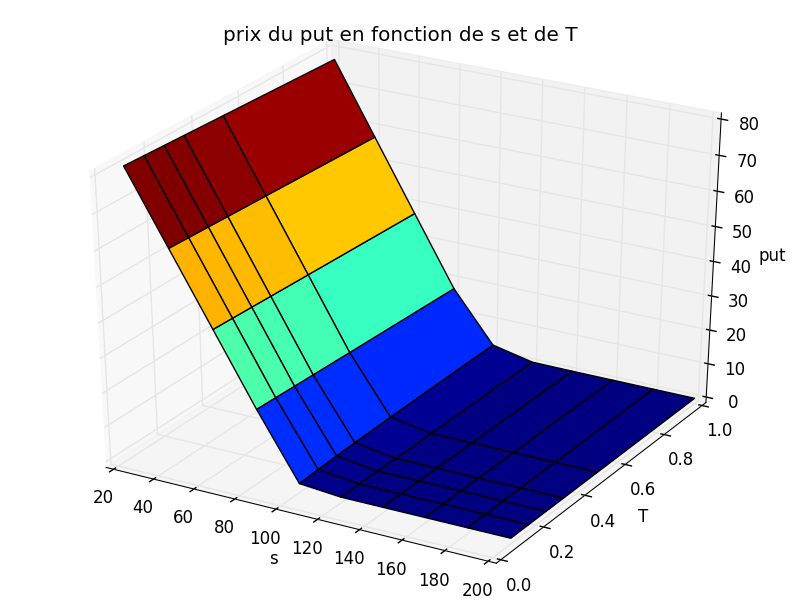
\includegraphics[height=9cm,keepaspectratio]{./images/Q18.png}
    \end{center}
    \caption{\textit{prix du put en fonction de $s$ et $T$}}
    \label{Q18}
  \end{figure}
  
  \newpage
  \section{Convergence des prix}
  \paragraph{19.} voir fichier `code/Q19.py`
  
  On remarque que le \textit{price1} semble converger vers le prix du \textit{put} pour $N >> 1$. Or à la question 17 nous avons vu que le pricer 3 convergait aussi vers le put. Donc ce graphe montre bien la convergence des prix dans le cas du modèle de Cox-Ross-Rubinstein(pricer1) vers les prix donnés dans le cas du modèle de Black-Scholes(pricer3).
  
  \begin{figure}[H]
    \begin{center}
      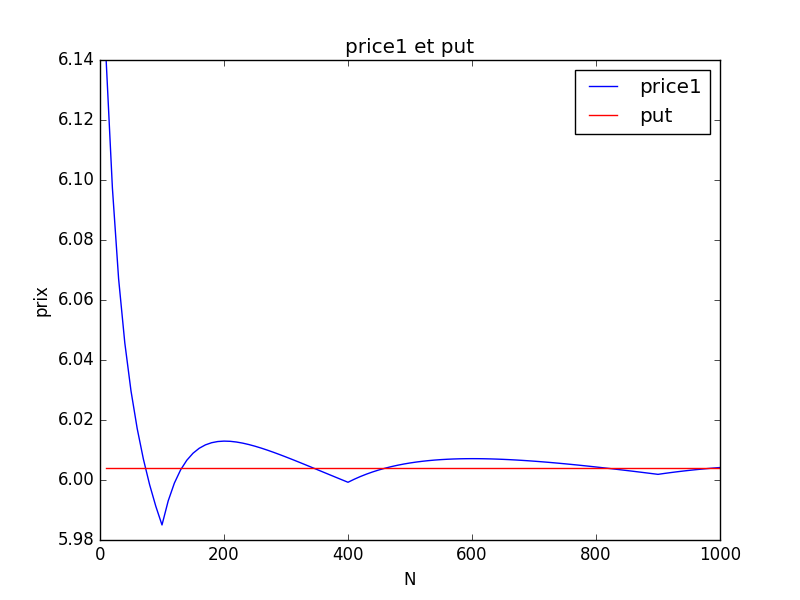
\includegraphics[height=9cm,keepaspectratio]{./images/Q19.png}
    \end{center}
    \caption{\textit{Price1 et put}}
    \label{Q19}
  \end{figure}
  
  \newpage
  \section{EDP de Black-Scholes}
  La fonction prix du put $P$ vérifie l'équation différentielle suivante $\forall t, S \in [0, T] \times [0, L]$:
  $$\frac{\partial P}{\partial t} + rS\frac{\partial P}{\partial S} + \frac{1}{2} \sigma^2 S^2 \frac{\partial^2 P}{\partial S^2} = rP$$
  
  Les conditions de bords nous donnent les valeurs de $P$ en:
  $$(T, s) \quad t.q \quad s \in [0, L]$$
  $$(t, 0) \quad t.q \quad t \in [0, T]$$
  $$(t, L) \quad t.q \quad t \in [0, T]$$
  
  Ce qui peut se représenter sur le plan suivant:
  
  On cherche à intégrer numériquement, afin d'obtenir une estimation des valeurs $P(0, s), \forall s \in [0, L]$.
  
  Pour cela, on discrétise le plan de la façon suivante. Soit $N, M \in \mathbb{N}^*$:
  
  $$
  \begin{sistema}
    \Delta T = \frac{T}{N} \quad et \quad \forall i \in \{0, ..., N\}, \boxed{t_i = i \Delta T}\\
    \Delta S = \frac{L}{M + 1} \quad et \quad \forall j \in \{0, ..., M + 1\}, \boxed{S_j = j \Delta S}
  \end{sistema}
  $$
  
  \begin{figure}[H]
    \begin{center}
      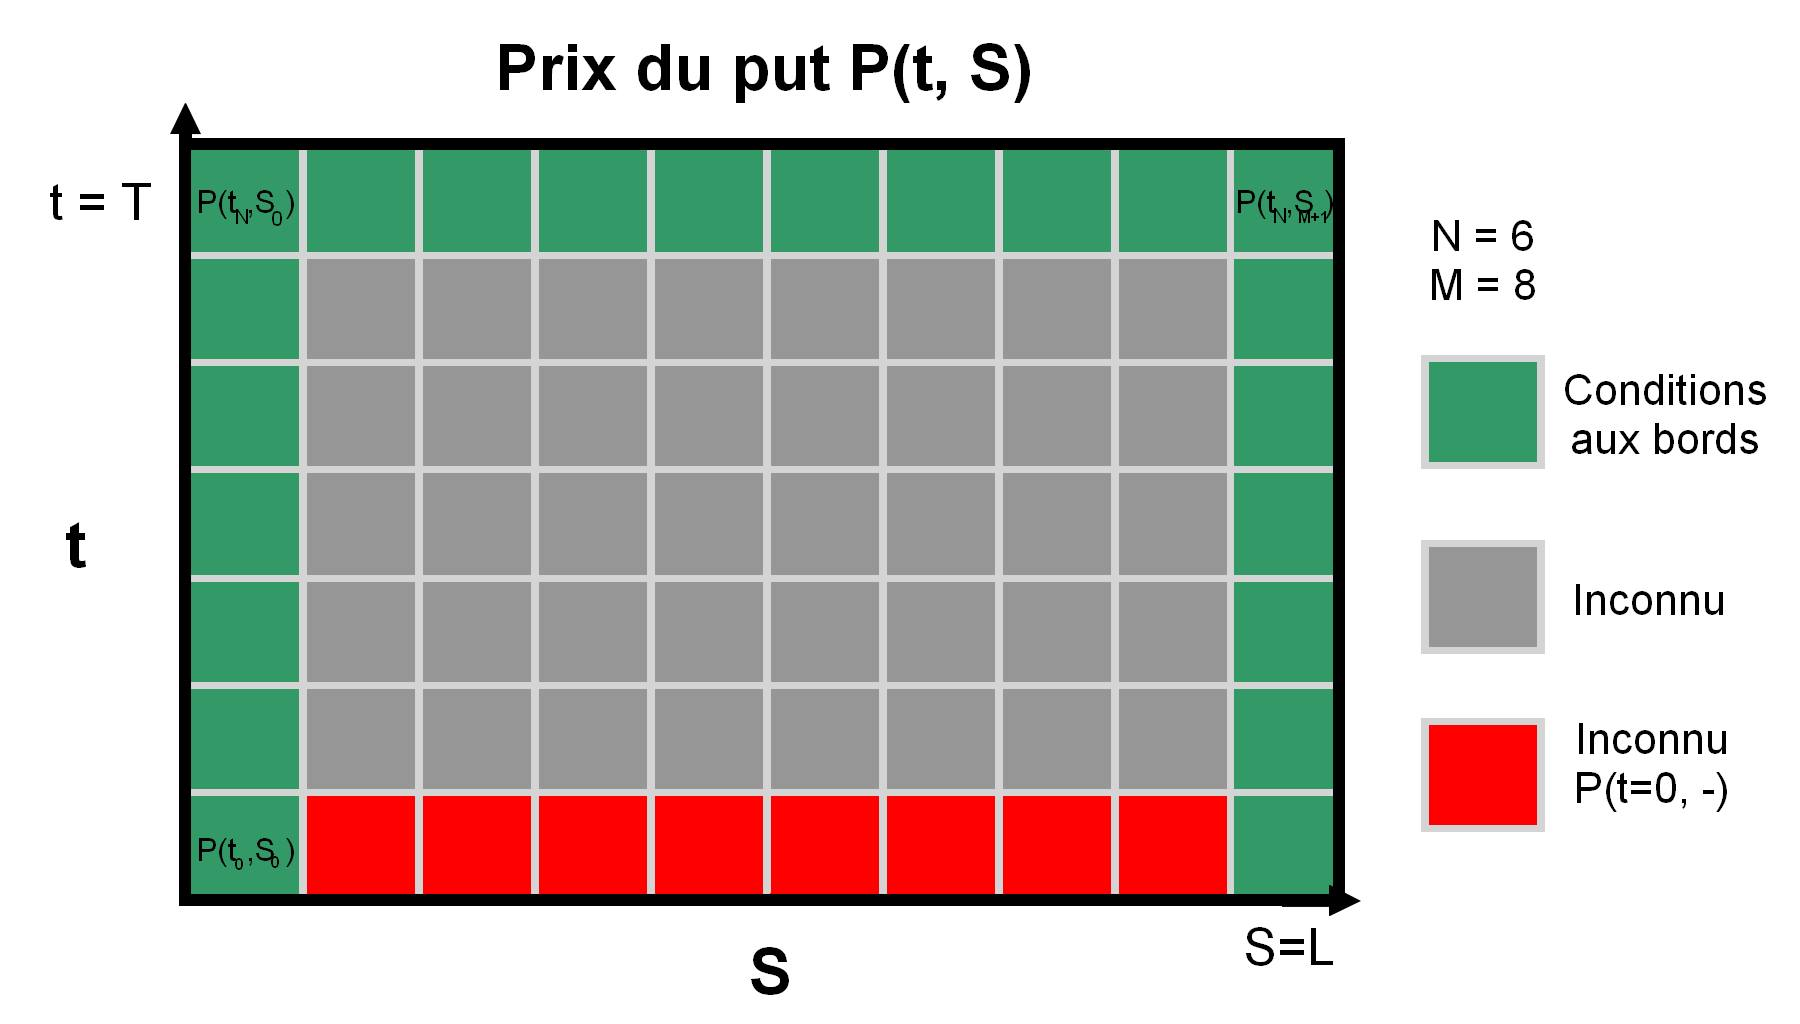
\includegraphics[height=9cm,keepaspectratio]{./images/edp.jpg}
    \end{center}
    \caption{\textit{Grille schématisant la résolution}}
    \label{grille}
  \end{figure}
  
  De plus, on effectue les approximations suivantes : $\forall (i, j) \in \{0, ..., N-1\} \times \{1, ..., M\}$ et $\forall \theta \in [0, 1]$:          
  $$
  \boxed{
    \begin{sistema}
      \frac{\partial P}{\partial t}(t_i, S_j) \simeq \frac{1}{\Delta T}\left(P(t_{i + 1}, s_j) - P(t_i, s_j)\right)\\
      \frac{\partial P}{\partial S}(t_i, S_j) \simeq \theta * \frac{P(t_{i + 1}, s_{j + 1}) - P(t_{i + 1}, s_j)}{\Delta S} + (1 - \theta) * \frac{P(t_i, s_{j + 1}) - P(t_i, s_j)}{\Delta S}\\
      \frac{\partial^2 P}{\partial S^2}(t_i, S_j) \simeq \theta * \frac{P(t_{i + 1}, s_{j + 1}) - 2P(t_{i + 1}, s_j) + P(t_{i + 1}, s_{j-1})}{\Delta S^2} + (1 - \theta) * \frac{P(t_{i}, s_{j + 1}) - 2P(t_{i}, s_j) + P(t_{i}, s_{j-1})}{\Delta S^2}
    \end{sistema}
  }
  $$
  \paragraph{Remarque}
  \begin{itemize}[label=-]
    \item Pour $\theta = 0$, on obtient un schéma d'Euler implicit
    \item Pour $\theta = 1$, on obtient un schéma d'Euler explicit
    \item Pour $\theta = \frac{1}{2}$, on obtient la méthode de Crank-Nicolson
  \end{itemize}
  
  En approximant l'équation différentielle $\forall (i, j) \in \{0, ..., N-1\} \times \{1, ..., M\}$ :
  
  $$
  \boxed{
    \frac{\partial P}{\partial t}(t_i, S_j) + r S_j \frac{\partial P}{\partial S}(t_i, S_j) + \frac{1}{2} \sigma^2 S_j^2 \frac{\partial^2 P}{\partial S^2}(t_i, S_j) = r P(t_{i + 1}, S_j)
  }
  $$
  
  après developpement et séparation des termes en $t_i$ et $t_{i+1}$, on obtient:
  \begin{framed} 
    \begin{align*}
      \left[\frac{1}{\Delta T} + \left(r \frac{S_j}{\Delta S} + \sigma^2 \frac{S_j^2}{\Delta S^2} \right) (1 - \theta)\right] P(t_i, S_j) \\
      - \left( r \frac{S_j}{\Delta S} + \frac{1}{2} \sigma^2 \frac{S_j^2}{\Delta S^2} \right) (1 - \theta) P(t_i, S_{j + 1}) \\
      - \frac{1}{2} \sigma^2 \frac{S_j^2}{\Delta S^2} (1 - \theta) P(t_i, S_{j - 1}) \\
      = \left[-r + \frac{1}{\Delta T} - \left(r \frac{S_j}{\Delta S} + \sigma^2 \frac{S_j^2}{\Delta S^2}\right) \theta \right] P(t_{i + 1}, S_j) \\
      + \left( r \frac{S_j}{\Delta S} + \frac{1}{2} \sigma^2 \frac{S_j^2}{\Delta S^2} \right) \theta P(t_{i + 1}, S_{j + 1}) \\
      + \frac{1}{2} \sigma^2 \frac{S_j^2}{\Delta S^2} \theta P(t_{i + 1}, S_{j - 1})
    \end{align*}
  \end{framed}
  
  $$\Leftrightarrow$$
  
  \begin{align*}
    A_{i, j} P(t_i, S_j) + A_{i, j+1} P(t_i, S_{j + 1}) + A_{i, j-1} P(t_i, S_{j - 1}) \\
    = B_{i + 1, j} P(t_{i + 1}, S_j) + B_{i+1, j+1} P(t_{i + 1}, S_{j + 1}) + B_{i+1, j-1} P(t_{i + 1}, S_{j - 1})
  \end{align*}
  
  Ce qui peut se représenter sous forme des systèmes linéaires suivant $\forall i \in \{0, ..., N-1\}$
  $$\boxed{A X_i = B X_{i+1} + C_i}$$
  \newpage
  avec:
  \begin{itemize}[label=-]
    \item $\forall i \in \{0, ..., N\}, X_i=$ \begin{pmatrix}P(t_i, S_0)\\...\\P(t_i, S_{M+1})\end{pmatrix} ($X_{N}$ est connu par les conditions initiales, on recherche à déterminer $X_0$)
    \item A (tridiagonale) = $
    \begin{blockarray}{ccccccccccc}
      0 & 1 & 2 & ... & j-1 & j & j+1 & ... & M & M+1 \\
      \begin{block}{(cccccccccc)c}
	A_{0, 0} & A_{0, 1} &     0    &  0   &    ...        &     ...      & ...        & ... & ...        &  0         & 0     \\
	A_{1, 0} & A_{1, 1} & A_{1, 2} &  0   &    ...        &     ...      & ...        & ... & ...        &  0         & 1     \\
	0        & A_{2, 1} &    ...   & ...  &    ...        &     ...      & ...        & ... & ...        & ...        & 2     \\
	0        &    0     &    ...   & ...  &    ...        &     ...      & ...        & ... & ...        & ...        & ...   \\
	...      &   ...    &    ...   & ...  &    ...        &     ...      & ...        & ... & ...        & ...        & j-1   \\
	...      &   ...    &    ...   & ...  &  A_{j, j-1}   &   A_{j, j}   & A_{j, j+1} & ... & ...        & ...        & j     \\
	...      &   ...    &    ...   & ...  &    ...        &     ...      & ...        & ... & ...        & ...        & j+1   \\
	...      &   ...    &    ...   & ...  &    ...        &     ...      & ...        & ... & ...        &  0           & ... \\
	...      &   ...    &    ...   & ...  &    ...        &     ...      & ...        & ... & ...        & A_{M, M+1}   & M   \\
	0        &    0     &    ...   & ...  &    ...        &     ...      & ...        &  0  & A_{M+1, M} & A_{M+1, M+1} & M+1 \\
      \end{block}
    \end{blockarray}
    $
    \begin{itemize}[label=-]
      \item $A_{0, 0} \quad \quad \quad  \quad = 1 $
      \item $A_{0, 1} \quad \quad \quad  \quad = 0 $
      \item $A_{M+1, M} \quad \quad            = 0 $
      \item $A_{M+1, M+1} \quad                = 1 $
      \item $\forall j \in \{1, ..., M\}$
      $
      \begin{sistema}
	A_{j, j-1} \quad = \quad        - \frac{1}{2} \sigma^2 \frac{S_j^2}{\Delta S^2} (1 - \theta) \\
	A_{j, j}   \quad \quad = \quad  \frac{1}{\Delta T} + \left(r \frac{S_j}{\Delta S} + \sigma^2 \frac{S_j^2}{\Delta S^2} \right) (1 - \theta) \\
	A_{j, j+1} \quad = \quad        - \left( r \frac{S_j}{\Delta S} + \frac{1}{2} \sigma^2 \frac{S_j^2}{\Delta S^2} \right) (1 - \theta)
      \end{sistema}
      $
      \item Tous les autres $A_{i, j} = 0$
    \end{itemize}
    \item B (tridiagonale) = $
    \begin{blockarray}{ccccccccccc}
      0 & 1 & 2 & ... & j-1 & j & j+1 & ... & M & M+1 \\
      \begin{block}{(cccccccccc)c}
	B_{0, 0} & B_{0, 1} &     0    &  0   &    ...        &     ...      & ...        & ... & ...        &  0         & 0     \\
	B_{1, 0} & B_{1, 1} & B_{1, 2} &  0   &    ...        &     ...      & ...        & ... & ...        &  0         & 1     \\
	0        & B_{2, 1} &    ...   & ...  &    ...        &     ...      & ...        & ... & ...        & ...        & 2     \\
	0        &    0     &    ...   & ...  &    ...        &     ...      & ...        & ... & ...        & ...        & ...   \\
	...      &   ...    &    ...   & ...  &    ...        &     ...      & ...        & ... & ...        & ...        & j-1   \\
	...      &   ...    &    ...   & ...  &  B_{j, j-1}   &   B_{j, j}   & B_{j, j+1} & ... & ...        & ...        & j     \\
	...      &   ...    &    ...   & ...  &    ...        &     ...      & ...        & ... & ...        & ...        & j+1   \\
	...      &   ...    &    ...   & ...  &    ...        &     ...      & ...        & ... & ...        &  0           & ... \\
	...      &   ...    &    ...   & ...  &    ...        &     ...      & ...        & ... & ...        & B_{M, M+1}   & M   \\
	0        &    0     &    ...   & ...  &    ...        &     ...      & ...        &  0  & B_{M+1, M} & B_{M+1, M+1} & M+1 \\
      \end{block}
    \end{blockarray}
    $
    \begin{itemize}[label=-]
      \item $B_{0, 0} \quad \quad \quad  \quad = 0 $
      \item $B_{0, 1} \quad \quad \quad  \quad = 0 $
      \item $B_{M+1, M} \quad  \quad           = 0 $
      \item $B_{M+1, M+1} \quad                = 0 $
      \item $\forall j \in \{1, ..., M\}$
      $
      \begin{sistema}
	B_{j, j-1} \quad = \quad        \frac{1}{2} \sigma^2 \frac{S_j^2}{\Delta S^2} \theta \\
	B_{j, j}   \quad \quad = \quad  -r + \frac{1}{\Delta T} - \left(r \frac{S_j}{\Delta S} + \sigma^2 \frac{S_j^2}{\Delta S^2}\right) \theta \\
	B_{j, j+1} \quad = \quad        \left( r \frac{S_j}{\Delta S} + \frac{1}{2} \sigma^2 \frac{S_j^2}{\Delta S^2} \right) \theta
      \end{sistema}
      $
      \item Tous les autres $B_{i, j} = 0$
    \end{itemize}
    \item $C_i$ conditions de bords = $
    \begin{blockarray}{cc}
      \begin{block}{(c)c}
	P(t_i, S_0)     &  0  \\
	0               &  1  \\
	...             & ... \\
	0               &  M  \\
	P(t_i, S_{M+1}) & M+1 \\
      \end{block}
    \end{blockarray}
    $
  \end{itemize}
  
  \paragraph{Remarque} Les valeurs de $A_{0, 0}, B_{0, 0}, B_{0, 1}, B_{M+1, M}, B_{M+1, M+1}, C_0, C_M$ ont été choisit de sorte à ce que l'équation
  $A X_i = B X_{i+1} + C_i$ soit vérifié pour les lignes $0$ et $M+1$. Ce sont les \textit{conditions initiales}.
  \newline
  \newline
  $X_{N}$ est determiné par les conditions initiales, on peut donc en déduire $X_{N-1}$, puis par récurrence sur le système,
  $X_i$ devient connu $\forall i \in \{0, ..., N - 1\}$.
  \newline
  \newline
  On a donc $N - 1$ systèmes linéaires : $\forall i \in \{0, ..., N - 1\}, A X_i = b_i$, avec $b_i = B X_{i+1} + C_i$,
  qu'il nous reste à résoudre dans l'ordre $i$ décroissant, afin d'obtenir $X_0$: approximation du prix du put $P(0, S)$ en $t=0, S \in [0, L]$
  
  \paragraph{Optimisation} $A$ est indépendante de $i$, on a donc uniquement à la générer une fois au début de la résolution.
  Avec une résolution par la méthode de Gauss (triangulation + résolution), on aurait une complexité temporelle en $\frac{2}{3}M^3 + o(M^3)$
  Or, $A$ est tridiagonale, on peut donc optimiser la résolution, et on atteinds une complexité temporelle en $8M + o(M)$ (factorisation LU + résolution) (voir \ref{tridiagonale} p.8-9)
  
  De plus, on gagne aussi en performance mémoire: $A$ tridiagonale peut être stocker en $3M + o(M)$ (de même pour $B$)
  
  \paragraph{Résolution}
  La résolution de ces systèmes (en Python) est réalisé avec la bibliothèque $scipy.linalg$ et $numpy$,
  qui propose une fonction optimisé de résolution de tels systèmes. (voir \ref{banded})
  \newline
  \newline
  Le code qui a généré les résultats suivant est disponible dans les fichiers 'code/EDP.py'.
  
  Voici l'algorithme en pseudo-code:
  \begin{algorithm}
    \caption{Résolution de l'équation différentielle de Black-Scholes}
    \begin{algorithmic}
      \REQUIRE $M, N \in \mathbb{N^*} , K, R, \sigma \in \mathbb{R}, \theta \in [0, 1]$
      \STATE $\delta T \leftarrow \frac{T}{N}$
      \STATE $\delta S \leftarrow \frac{T}{M + 1}$
      \STATE Initialiser les matrices $A$ et $B$ (avec $K, R, \sigma, \theta, \delta T$ et $\delta S$)
      \STATE Initialiser $X_N$ (conditions aux bords)
      \FOR{$i := N - 1$ ; $i >= 0$ ; $i := i - 1$}
	\STATE Calculer $b_i \leftarrow B.X_{i + 1} + C_{i}$
	\STATE Résoudre systeme triangulaire : $X_i := solve(A . X_i = b_i)$
      \ENDFOR
      \STATE Renvoyer $X_0$
    \end{algorithmic}
  \end{algorithm}

  
  \newpage
  Pour les méthodes \textbf{implicit} et de \textbf{Crank Nicholson}, la méthode est toujours \textbf{stable} (voir \ref{finite})
  On obtient une erreur relative entre les 2 solutions:
  \begin{figure}[H]
    \begin{center}
      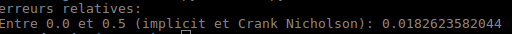
\includegraphics[width=12cm,keepaspectratio]{./images/erreur_implicit_crank-nicholson_1000_1000.png}
    \end{center}
    \caption{\textit{Erreur relative entre les 2 solutions obtenus}}
    \label{erreur_1000_1000}
  \end{figure}
  
  On obtient les solutions suivantes pour le prix du put à $t=0$:
  \begin{figure}[H]
    \begin{center}
      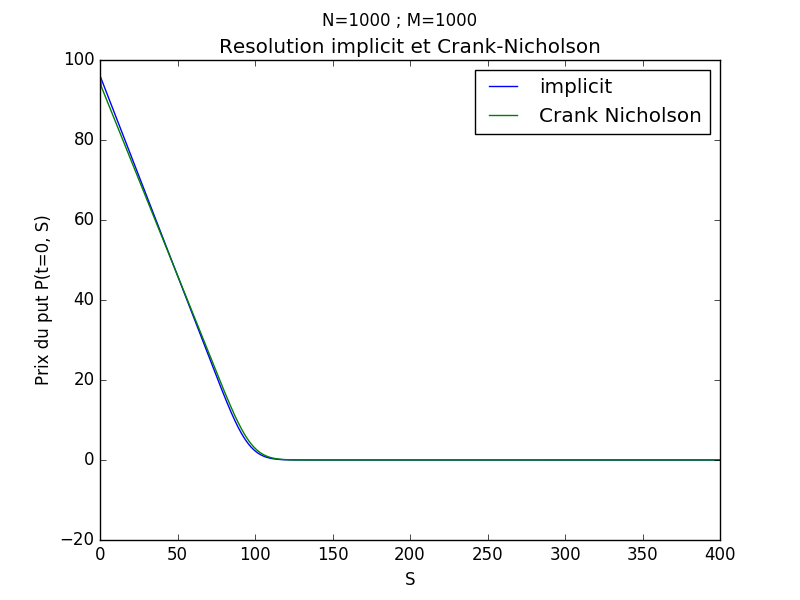
\includegraphics[height=7cm,keepaspectratio]{./images/implicit_crank-nicholson_1000_1000.png}
    \end{center}
    \caption{\textit{Solutions obtenus par méthode implicit et Crank-Nicholson}}
    \label{implicit_crank-nicholson_1000_1000}
  \end{figure}
  
  \begin{figure}[H]
    \begin{center}
      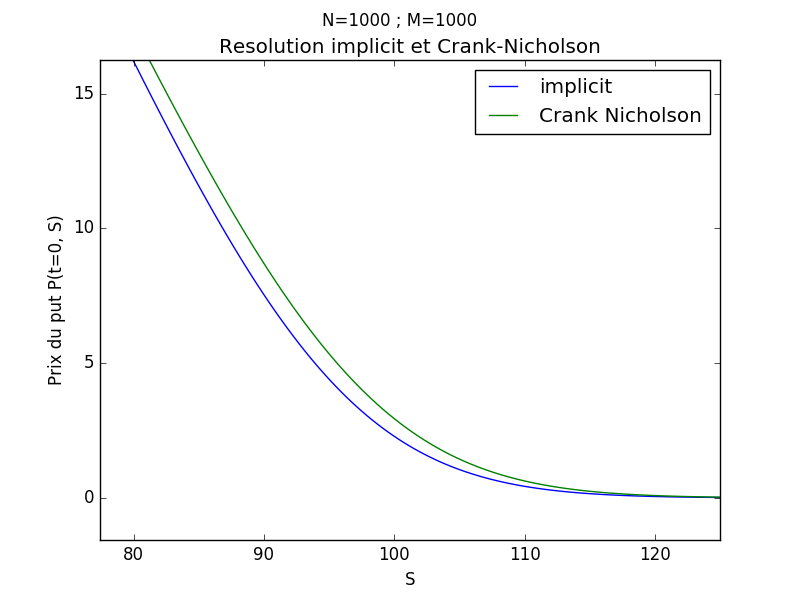
\includegraphics[height=7cm,keepaspectratio]{images/implicit_crank-nicholson_1000_1000_zoom.png}
    \end{center}
    \caption{\textit{Solutions obtenus par méthode implicit et Crank-Nicholson (zoomées)}}
    \label{implicit_1000_1000}
  \end{figure}
  
  
  \newpage
  Pour la méthode \textbf{explicit}, le schéma est stable si le pas de temps est de l'ordre du carré du pas d'espace.
  Autrement dit, si: $$\Delta t \simeq \Delta S^2$$
  
  On observe cette instabilité pour $M = N = 296$ (voir 'code/Q20/EDP\_296\_296.py'):
  
  \begin{figure}[H]
    \begin{center}
      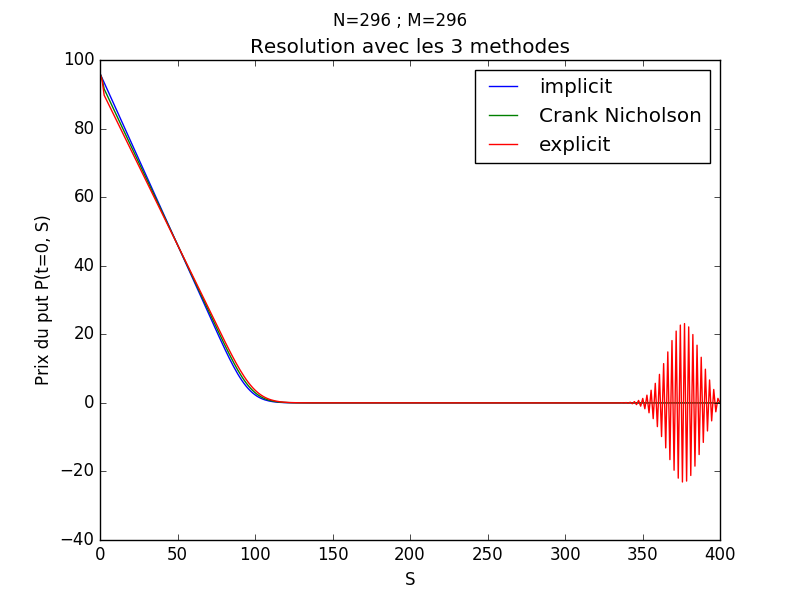
\includegraphics[height=8cm,keepaspectratio]{./images/explicit_implicit_cranknicholson_296_296.png}
    \end{center}
    \caption{\textit{Solution avec les 3 méthodes}}
    \label{explicit_implicit_cranknicholson_296_296}
  \end{figure}
  
  \begin{figure}[H]
    \begin{center}
      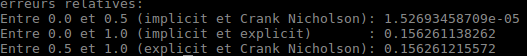
\includegraphics[width=12cm,keepaspectratio]{./images/erreurs_296_296.png}
    \end{center}
    \caption{\textit{Erreur relative entre les 3 méthodes pour $M=N=296$}}
    \label{erreurs_296_296}
  \end{figure}
  
  \begin{figure}[H]
    \begin{center}
      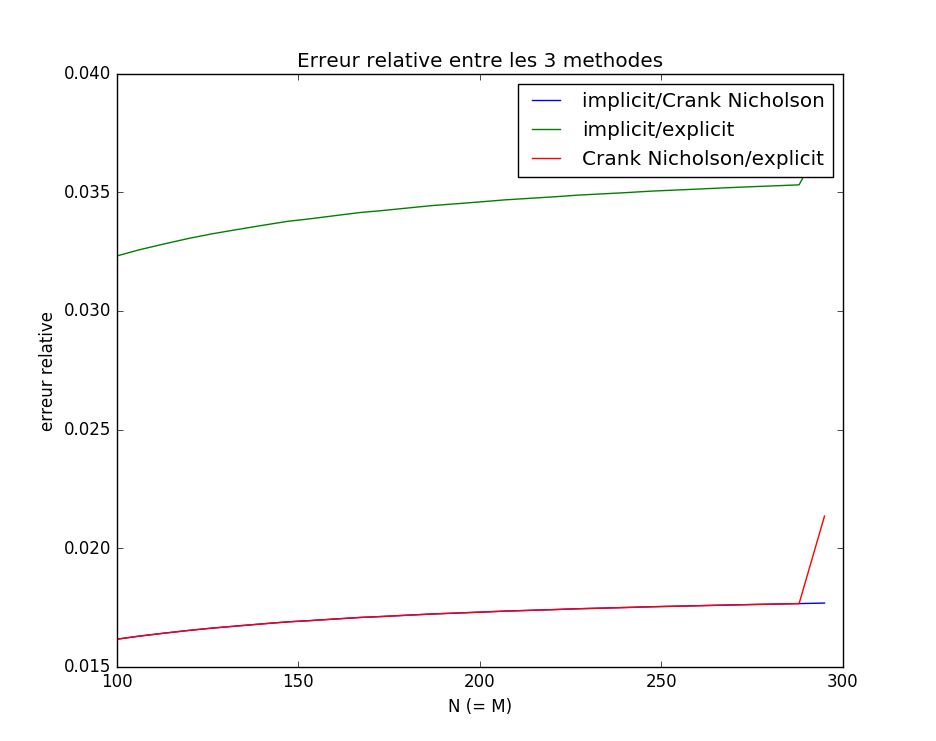
\includegraphics[width=12cm,keepaspectratio]{./images/edp_err.png}
    \end{center}
    \caption{\textit{Erreur relative entre les 3 méthodes pour $M=N \in [100, 296]$}}
    \label{edp_err}
  \end{figure}
  
  On en déduit que lorsque les 3 méthodes convergent, elles donnent des résultats très proches.
  Pour $M$ plus grand que $296$, la diverge de la méthode explicit fait exploser l'erreur relative.
  
  \newpage
  Pour $M = 1000$ et $N=M^2$, la méthode explicit est stable et on obtient la solution suivante (voir 'code/Q20/EDP\_1000\_1000000.py'):
  
  \begin{figure}[H]
    \begin{center}
      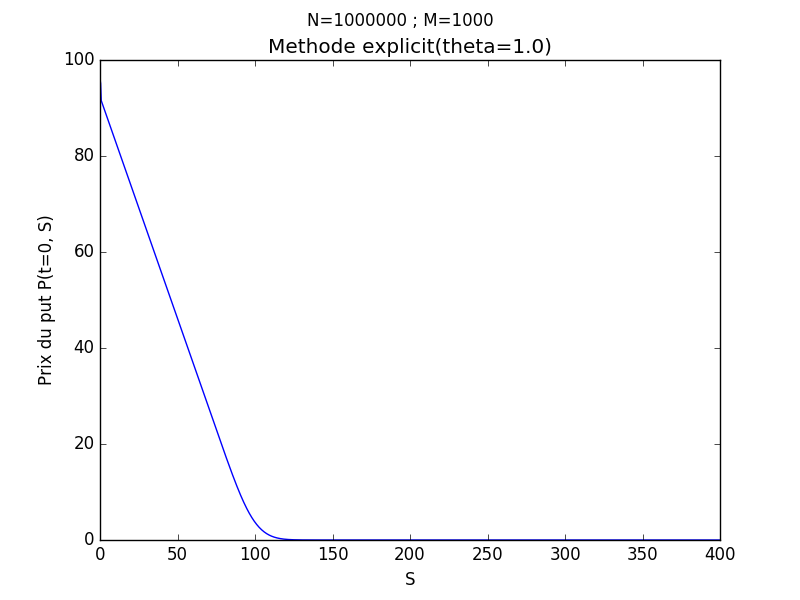
\includegraphics[height=8cm,keepaspectratio]{./images/explicit_1000_1000000.png}
    \end{center}
    \caption{\textit{Solution explicit avec un rapport quadratique sur les pas}}
    \label{explicit_1000_1000000}
  \end{figure}
  
  \begin{figure}[H]
    \begin{center}
      
\includegraphics[width=12cm,keepaspectratio]{./images/temps_explicit_1000.png}
    \end{center}
    \caption{\textit{Temps d'execution de la résolution explicit pour $M=1000$ et $N=M^2$ précèdente (15m47s)}}
    \label{temps_explicit_1000}
  \end{figure}
  
  \newpage
  \paragraph{Expression approchée}
  Finalement, en guise de \textbf{bonus}, on se propose d'obtenir une expression approchée du prix du put $P(t=0, S)$.
  Pour cela, et d'après l'allure des figures, on se propose d'approcher cette fonction par le modèle exponentielle suivant (voir 'code/Q20/EDP\_Modele\_exponentielle.py'):
  
  $$\boxed{P(t=0, S) = a e^{-bS^3 - cS + d} + e \quad t.q. \quad a, d, e \in \mathbb{R} \quad et \quad b, c \in \mathbb{R^*_+}}$$
  
  Grâce aux modules 'numpy' et 'scipy' de Python, on a pu obtenir un modèle rapidement (voir curve\_fit \ref{curve_fit}):
  
  \begin{figure}[H]
    \begin{center}
      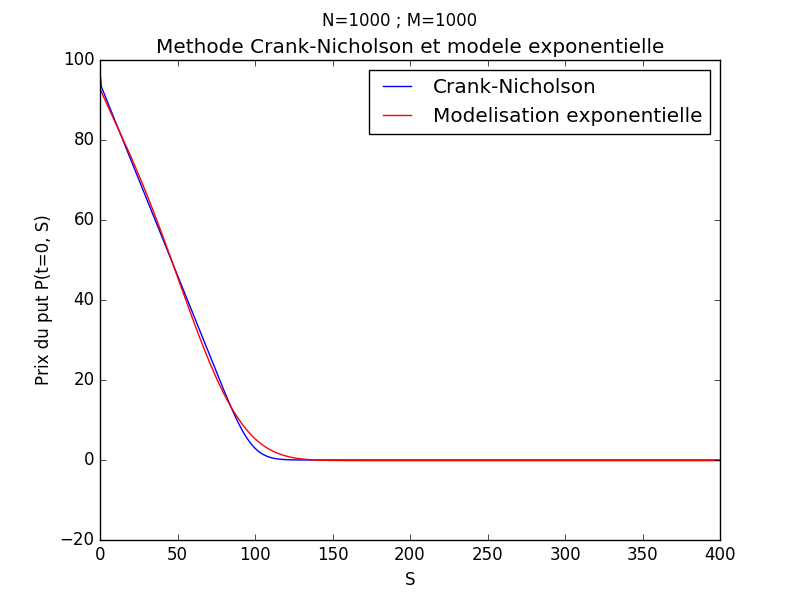
\includegraphics[height=8cm,keepaspectratio]{./images/modele_exp.png}
    \end{center}
    \caption{\textit{Modèle exponentielle obtenu}}
    \label{modele_exp}
  \end{figure}
  
  \begin{figure}[H]
    \begin{center}
      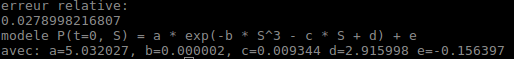
\includegraphics[width=12cm,keepaspectratio]{./images/modele_exp_vars.png}
    \end{center}
    \caption{\textit{Erreur relative et paramètre optimal obtenu, entre le résultat obtenu par la méthode de Crank-Nicholson et le modèle exponentielle}}
    \label{modele_exp_vars}
  \end{figure}
  
  \newpage
  
  \section{Références}
  \begin{thebibliography}{}
    
    \bibitem{tridiagonale}\label{tridiagonale}
    'Analyse Numérique' - Paola GOATIN\newline
    \href{https://team.inria.fr/opale/files/2011/11/Anum.pdf}
    {\textit{https://team.inria.fr/opale/files/2011/11/Anum.pdf}}
    \newline
    \bibitem{banded}\label{banded}
    'Résolution de système linéaires 'en bande' - SCIPY\newline
    \href{https://docs.scipy.org/doc/scipy/reference/linalg.html}
    {\textit{https://docs.scipy.org/doc/scipy/reference/linalg.html}}
    \newline
    \bibitem{finite}\label{finite}
    'Finite difference method' - Wikipédia\newline
    \href{https://en.wikipedia.org/wiki/Finite\_difference\_method}
    {\textit{https://en.wikipedia.org/wiki/Finite\_difference\_method}}
    \newline
    \bibitem{curve_fit}\label{curve_fit}
    scipy.optimize.curve - Documentation scipy\newline
    \href{https://docs.scipy.org/doc/scipy/reference/generated/scipy.optimize.curve\_fit.html}
    {\textit{https://docs.scipy.org/doc/scipy/reference/generated/scipy.optimize.curve\_fit.html}}
    
    
  \end{thebibliography}
  
\end{document}
